\documentclass[conference]{IEEEtran}
\IEEEoverridecommandlockouts

\usepackage{cite}
\usepackage{amsmath,amssymb,amsfonts}
\usepackage{algorithmic}
\usepackage{graphicx}
\usepackage{textcomp}
\usepackage{xcolor}
\def\BibTeX{{\rm B\kern-.05em{\sc i\kern-.025em b}\kern-.08em
    T\kern-.1667em\lower.7ex\hbox{E}\kern-.125emX}}
\begin{document}

\title{Inteligência Artificial no Processo de Seleção de Candidatos a Vagas de Emprego\\

}



\author{\IEEEauthorblockN{1\textsuperscript{st} Francisca Amanda Miranda de Paula}
\IEEEauthorblockA{\textit{Centro Universitário IESB} \\
\textit{Centro Universitário Instituto de Educação Superior de Brasília}\\
Brasília, Brasil \\
Matrícula - 1812082052}
\and
\IEEEauthorblockN{2\textsuperscript{nd} Matheus Henrique Santos Lucas}
\IEEEauthorblockA{\textit{Centro Universitário IESB} \\
\textit{Centro Universitário Instituto de Educação Superior de Brasília}\\
Brasília, Brasil \\
Matrícula - 1822082032}
\and
\IEEEauthorblockN{3\textsuperscript{rd} João Victor Resende}
\IEEEauthorblockA{\textit{Centro Universitário IESB} \\
\textit{Centro Universitário Instituto de Educação Superior de Brasília}\\
Brasilia, Brasil \\
Matrícula - 1712130023}
}

\maketitle

\begin{resumo}
O presente projeto consiste em desenvolver um aplicativo na linguagem flutter, que inclui técnicas de inteligência artificial para selecionar automaticamente o candidato que se encaixar melhor com a oportunidade de emprego. Para o desenvolvimento da aplicação, com o objetivo de ter um projeto mais limpo, organizado e fácil de receber manutenção, foram implementados alguns recursos, sendo eles: arquitetura limpa (Clean Architecture), padrão de projeto MVVM, spring boot e lombok na API em Java etc.
\end{resumo}

\begin{IEEEpalavrachave}
inteligência artificial
\end{IEEEpalavrachave}

\begin{abstract}
The present project consists in developing an application in flutter language, that includes techniques of artificial intelligence to automatically select the candidate who best fits the job opportunity. For application development, with the goal to have a cleaner project, more organized and easier to receive maintenance, was implemented some resources, like: clean architecture (Clean Architecture), MVVM design pattern, spring boot and lombok frameworks in the API in the Java etc.
\end{abstract}

\begin{IEEEkeywords}
artificial intelligence
\end{IEEEkeywords}

\section{Introdução}
O uso da inteligência artificial dentro da área de recursos humanos traz muitos benefícios ao agilizar o processo de contratação, além de torná-los mais eficazes. 

\section{Contextualização}

A candidatura às vagas de emprego geralmente é bastante concorrida tendo muitos participantes para fazer a avaliação do perfil, tornando o processo de contratação lento na maioria das vezes. Sendo assim, é interessante agilizar o processo de seleção, visto que a demora pode prejudicar tanto a empresa quanto os interessados pela vaga.

Portanto, muitas empresas quando estão contratando, ficam com certas demandas paradas somente esperando o novo funcionário assumir o cargo para então dar andamento e prosseguimento às tarefas, sendo que até o novo funcionário se adaptar às atividades leva algum tempo, o que pode levar ao atraso do cumprimento das demandas e regressão na produtividade da equipe como um todo. Quanto ao candidato, este permanece disponível para o mercado de trabalho por mais tempo do que deveria, perdendo até outras oportunidades de emprego. 

\section{Problema}
Definir a melhor estratégia e técnica da inteligência artificial para usá-la na pré-seleção de candidatos em uma vaga específica, além de decidir quais variáveis serão levadas em conta para análise e tomada de decisão, obtendo uma alta taxa de precisão. Neste contexto, como selecionar o melhor candidato com a menor taxa de erros possíveis, tendo em vista que a quantidade de parâmetros para medir as habilidades de um profissional, considerando também os requisitos, são praticamente infinitos?

\section{Objetivo Geral}
Desenvolver um aplicativo para dispositivos móveis com sistema operacional Android, que faz uso da inteligência artificial para realizar uma contratação inicial de candidatos em vagas de emprego. Assim, para resolver o problema exposto, será necessário utilizar um algoritmo que faz ligação de variáveis, para comparar os atributos do perfil candidato com os atributos de requisito das vagas. Portanto uma das técnicas estudada que atende melhor o objetivo final do projeto para se obter os resultados esperados, é o algoritmo de regressão linear da área de inteligência artificial.

\section{Objetivos Específicos}
\begin{itemize}
\item Desenvolver e consumir APIs; 
\item Usar padrões de projeto e boas práticas de programação, como os princípios S.O.L.I.D e Clean Architecture; 
\item Planejar e criar a interface do usuário;
\item Integrar o backend com a Interface do usuário (frontend); 
\item Desenvolver funcionalidades para cadastro e autenticação de usuários;
\item Conectar no banco de dados PostgreSQL;
\item Subir aplicação para o Heroku;
\item Aplicar a inteligência artificial para a tomada de decisão e ligação de variáveis;
\item Incluir chat bot e mapa no projeto.
\end{itemize}

\section{Referencial Teórico}
É possível perceber que a inteligência artificial está cada vez mais presente dentro das empresas, porém, o seu processo de aplicação em uma determinada área pode ser complexo e lento a depender da forma como é feito a coleta de dados e o treinamento da IA. Algumas das técnicas de inteligência artificial, que podem ser aplicadas na área de recursos humanos para selecionar interessados em uma vaga de emprego, são: Lógica Fuzzy, Sistema Especialista, Redes Neurais Artificiais, Sistemas Baseados em Casos, Algoritmos de Classificação e Regressão Linear etc.

O uso de Redes Neurais Artificiais (RNA) auxilia o RH pelo motivo de ter a capacidade de prever os candidatos que seriam os mais adequados às vagas, além de ter uma enorme habilidade em aprender no ambiente em que está inserido. Assim, o RNA, com o aumento das informações que adquire ao longo das avaliações dos currículos dos candidatos, cada vez mais a sua escolha se tornará mais assertiva, pois ele aprende com base na experiência.

Já o método denominado como Sistema Especialista, consiste em um sistema que se comporta como um ser humano experiente em uma determinada área de atuação, podendo ser utilizado para fazer o papel de um especialista em RH. No Sistema Especialista, inicialmente é feita a coleta de dados a partir de um profissional experiente na sua área de atuação para que ele possa transmitir os seus conhecimentos para o sistema especialista. Logo em seguida, é criada uma base de conhecimento ou regras e, a partir disso, ela consegue fazer a inferência e dedução de novos conhecimentos sendo utilizada para a tomada de decisão, como decidir se vai selecionar ou não um candidato à vaga. 

Entretanto, apesar das técnicas mencionadas acima funcionarem muito bem, o Algoritmo de Regressão Linear é o mais adequado para o tema proposto. Como a técnica de análise de perfil para seleção envolve a comparação entre variáveis em que existe uma boa associação entre os dados, sendo elas as habilidades do candidato (Y) e os requisitos das vagas de emprego (X), a regressão linear verifica o quanto uma variável independente X está relacionada à outra variável dependente Y, fazendo um ajuste linear nos pontos do eixo (x,y), conforme mostra imagem abaixo:

\vspace{7mm}
\centerline{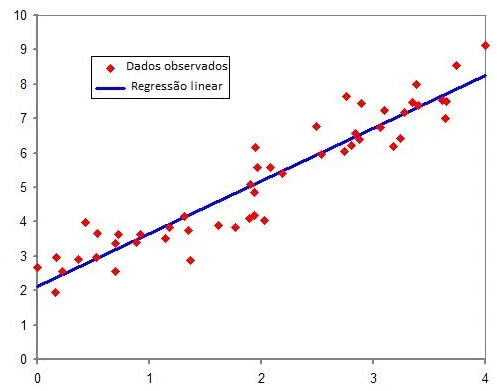
\includegraphics[width=80mm,height=600mm,keepaspectratio]{ExRegressaoLinear.png}}
\vspace{7mm}

\section*{Trabalhos Correlatos}
Entre inúmeras tecnologias existentes que automatizam processos, existem as que auxiliam no processo de contratação de candidatos às vagas de emprego. Como por exemplo, tem-se a ferramenta HireVue que é utilizada nas entrevistas online, sendo capaz de interpretar a análise da linguagem corporal, expressões faciais e tom de voz. Como estratégia de avaliação para decidir se o candidato é bom ou ruim, o entrevistado é comparado com os melhores funcionários da empresa, e a partir disso, selecionam os melhores para os recrutadores.

\section*{Metodologia}
A implementação do projeto é dividida em duas partes, sendo elas o aplicativo e a API. Para o desenvolvimento da API, foi utilizada a linguagem de programação Java, incluindo os frameworks spring boot e lombok. Já a parte do aplicativo, foi desenvolvido na linguagem flutter e para que ele rode no projeto, é necessário executar o seguinte comando no terminal, dentro da pasta onde fica o projeto:

\vspace{3mm}
\centerline{flutter pub get}
\vspace{3mm}

Este projeto poderá ser rodado nas IDE`s Visual Studio Code e no IntelliJ IDEA.

Para o armazenamento e manutenção dos dados, foi utilizado um banco de dados relacional PostgreSQL. Contudo, o projeto foi projetado para criar as tabelas de forma automática no momento da execução do programa, sem a necessidade de cria-las no banco usando o comando “Create Table”.

Com isso, as entidades da tabela foram definidas na pasta “entities”, sendo que cada arquivo representa uma tabela e os seus atributos indicam os campos desta entidade. Portanto, no momento da execução da API, a estrutura das tabelas ficará semelhante da forma que foi definida no algoritmo.

Sendo assim, foi utilizado o framework hibernate para a criação e alteração das tabelas no banco de dados, adicionando as seguintes informações no arquivo “application.properties”:

\vspace{7mm}
\centerline{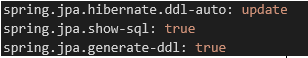
\includegraphics{AlgoritmoHibernate.png}}
\vspace{7mm}

Além disso, devem ser colocadas neste mesmo arquivo, os dados para se conectar no banco:

\vspace{7mm}
\centerline{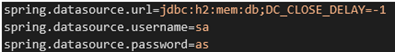
\includegraphics[width=80mm,height=600mm,keepaspectratio]{Postegresql.png}}
\vspace{7mm}

Com todos os pontos mencionados acima estando definidos, qualquer operação feita na API (criar, deletar, alterar, atualizar), será refletida automaticamente no banco de dados.

No projeto em Java, existe uma classe que é responsável por rodar a API, denominada Application. Já no app, a sua execução fica em um arquivo com a extensão “.main”.

\section*{Resultados Obtidos}



\section*{Conclusão}
Com o trabalho proposto, foi possível aprender como desenvolver um aplicativo móvel, usando boas práticas de programação, além de compreender melhor o funcionamento da inteligência artificial aplicada no processo de seleção de candidatos.

\section*{Cronograma Completo}

\begin{itemize}
\item 23/03 - 30/03:
\subitem Criação do repositório no github;
\subitem Levantamento de requisitos;
\subitem Diagramação de classes;
\subitem Definição da arquitetura e do padrão de projeto a ser utilizado;
\item 31/03 - 09/04:
\subitem Desenvolvimento das APIs;
\subitem Desenvolvimento da primeira parte do artigo;
\subitem Desenvolvimento da interface do usuário;
\subitem Criação das telas (onboarding, login, alteração de senha e cadastro de usuário);
\item 10/04 - 27/04:
\subitem Gestão de dependências;
\item 28/04 - 04/05:
\subitem Criação das telas específicas do tema do projeto;
\item 05/05 - 11/05: 
\subitem Consumo das APIs e integração com a interface do usuário;
\subitem Definição da estrutura de relacionamento das tabelas no banco de dados PostgreSQL;
\subitem Adição de mapa no aplicativo;
\item 12/05 - 18/05:
\subitem Desenvolvimento das funcionalidades de cadastro e autenticação de usuários; 
\subitem Criação de chat bot usando Dialogflow;
\item 19/05 - 15/06:
\subitem Uso da inteligência artificial no aplicativo;
\subitem Desenvolvimento da segunda parte do artigo.
\end{itemize}

\begin{thebibliography}{00}
\bibitem{b1} F. Bo-Shone, "Technology, Jobs e the Future of Work in Australia", Julho 2021.
\bibitem{b2} M. Afonso Paulo, R. Brenno Anderson, A. Cristine Amora e V. Rosângela Couras, "INTELIGÊNCIA ARTIFICIAL - RECURSOS HUMANOS FRENTE AS NOVAS TECNOLOGIAS, POSTURAS E ATRIBUIÇÕES", Outubro 2018.
\bibitem{b4} T. Ivana, "The Attitude of Job Candidates towards Artificial Intelligence in Hiring Process", Maio 2020.
\bibitem{b5} S. Abhilasha e S. Apurva, "Impact of Artificial Intelligence on HR practices in the UAE".
\bibitem{b6} R. Geetha e D. Bhanu Sree, "RECRUITMENT THROUGH ARTIFICIAL INTELLIGENCE: A CONCEPTUAL STUDY ".
\bibitem{b7} J. Mariana Namen, "INTELIGÊNCIA ARTIFICIAL NO RECRUTAMENTO and SELEÇÃO:INOVAÇÃO E SEUS IMPACTOS PARA A GESTÃO DE RECURSOSHUMANOS", Fevereiro 2020.
\end{thebibliography}
\vspace{12pt}

\end{document}
